\documentclass[12pt]{article} % \documentclass{} is the first command in any LaTeX code.  It is used to define what kind of document you are creating such as an article or a book, and begins the document preamble

\usepackage{amsmath} % \usepackage is a command that allows you to add functionality to your LaTeX code

\usepackage[papersize={216mm,330mm},tmargin=20mm,bmargin=20mm,lmargin=20mm,rmargin=20mm]{geometry}
\usepackage[english]{babel}
\usepackage[utf8]{inputenc}
\usepackage{amsmath,amssymb,mathabx,amsthm}%\for eqref
\usepackage{lscape}
\usepackage{graphicx}
\usepackage{tikz}\usetikzlibrary{arrows.meta,calc} %library tikz
\usepackage{subcaption}


\usepackage{pgfplots}
\pgfplotsset{compat=1.15}
\usepackage{mathrsfs}
\usetikzlibrary{arrows}

\usepackage{color,soul} %package for highlining
\usepackage[colorinlistoftodos]{todonotes}
\usepackage{fancyhdr}
\usepackage{hyperref} %creat hyperlink
\hypersetup{
    colorlinks=true,
    linkcolor=blue,
    filecolor=magenta,      
    urlcolor=cyan,
    pdftitle={Overleaf Example},
    pdfpagemode=FullScreen,
    } %set up a hyperlink to be in blue 
\newtheorem{theorem}{Theorem}
\newtheorem{definition}{Definition}[section]
\newtheorem{prop}[definition]{Proposition}
\newtheorem{lemma}[definition]{Lemma}
\newtheorem{example}[definition]{Example}

\newtheorem*{remark}{Remark}

\pagestyle{fancy}
\cfoot{\thepage} % this is for the page numbering
\setlength\parindent{0pt} % noindent for the whole document.
\renewcommand{\baselinestretch}{1.1} % increase the distance between line.

\DeclareMathOperator{\SLn}{\text{SL}_n(\mathbb{R})}
\DeclareMathOperator{\slnz}{SL_n(\mathbb{Z})}
\DeclareMathOperator{\glnz}{GL_n(\mathbb{Z})}
\DeclareMathOperator{\vol}{vol}

\DeclareMathOperator{\SO}{SO_n(\mathbb{R})}



\title{CHAPTER  :SEMI-STABLE LATTICE IN HIGHER RANK} % Sets article title
\date{\today} % Sets date for date compiled
\begin{document}
\maketitle % creates a title using the information in the preamble (title, author, date)
In this chapter, we will establish the notion of semi-stable lattice. Heuristically,
this is the lattice that achieve all the successive minima at the same time, see \cite{}.

We will provide two different definitions of semi -stable lattice: one is geometric - which follows Grayson's idea of utilizing
the canonical plot, and one is purely algebraic, which make use of the maximal standard parabolic subgroups.
The toy model will be the moduli space of 2-dimensional lattice, which is essential the upper half plane in the complex field.
At the end, we will show that the two definitions coincide.
\section{Lattices in higher rank}
For each $z$ with $\Im(z)>0$, we can attach to $z$ a lattice structure $L_z = \mathbb{Z}z \oplus \mathbb{Z}$. Roughly speaking
a lattice is a discrete  subgroup that is generated by a $k-$ basis of the $k$-space $V$.
In particular, we will only work with the real vector space $V$. Grayson works with lattice over a ring of algebraic integers, but we will restrict to
just the lattice that has the underlying structure as a $\mathbb{Z}-$ module.


The precise definition
of a lattice is as follows:
\begin{definition}[\label = Euclidean $\mathbb{Z}$-lattices]
    Let $L$ be a finitely generated $\mathbb{Z}$-module. In particular, it is a free $\mathbb{Z}$-module
    of finite rank. Suppose that $P$ is endowed with a real-valued symmetric positive definite\footnote{The non-degenerate implicity state that rank L is the same as $dim L_\mathbb{R}$} bilinear form, called $Q$.
    Then the space $L_\mathbb{R}= L \otimes_\mathbb{Z} \mathbb{R}$ equipped with the bilinear form $Q$ forms a real
    inner product space. We will call  the pair $(L,Q)$ a \textbf{Euclidean $\mathbb{Z}$-lattice}.
\end{definition}
\todo{add proof showing $L$ is a lattice in the second definition}

If there is no further confusion, we can just denote a Euclidean lattice by $L$, without specifying the bilinear form
$Q$. The lattice $l$ determines a full-rank lattice inside $L_\mathbb{R}$, namely, the rank
of the lattice $L$ is equal to the dimension of $L_\mathbb{R}$. We first recall the definition of discrete subgroup
\begin{definition}
    Let $V$ be a finite-dimensional vector space over $\mathbb{R}$, endowed with the natural topology. A subgroup $L$ of the additive group underlying the vector space $V$ is said to be \textit{discrete} if each point $y$ in $L$ has a neighbourhood in $V$ whose intersection with $L$ is $\{y\}$ or, equivalently, if, given a bounded set $C$ in $V$, the set $C \cap L$ is finite.
\end{definition}
Thus, using the following Proposition, $L$ has a structure of a discrete subgroup $V = L_\mathbb{R}$.
\begin{prop}
    Given a finite-dimensional vector space $V$ over $\mathbb{R}$, let $L$ be a subgroup of the additive group $V$, and let $m$ be the dimension of the $\mathbb{R}$-span of $L$ in $V$. Then $L$ is a discrete subgroup if and only if $L$ is a free abelian group of rank $m$.
\end{prop}
A proof can be found in \cite{}.
We now can define the notion of covolume of a lattice:
\begin{definition}[\label = Volume]\label{volume}
    Let's assume that $L$ is a full-rank lattice and has a basis
    \[L = \mathbb{Z}l_1 \oplus \ldots \oplus\mathbb{Z}l_n\]
    Then the volume of this lattice is defined to be the volume of the fundamental
    parallepiped. In particular, let $\left\lbrace e_i\right\rbrace$ be any orthonormal
    basis of the vector space $V = L_\mathbb{R}$. Then
    \[\vol(L) := \left|\det Q(l_i,e_j)\right|\]
\end{definition}
However, for the sake of computation, we also usually adopt another definition of the lattice.
In particular, we view lattice as a free $\mathbb{Z}-$ module of rank $n$ that is isomorphic
to $\mathbb{R}^n$ via base changing.
In more detail
\begin{definition}\label{lattice2}
    A \textit{lattice} in $\mathbb{R}^n$ is a subset $L \subset \mathbb{R}^n$ such that there exists
    a basis $b_1,\ldots,b_n$ of $\mathbb{R}^n$ such that
    \[L = \mathbb{Z}b_1\oplus \mathbb{Z}b_2\oplus \ldots \mathbb{Z}b_n\]
    If we put the vector $b_1,b_2,\ldots,b_n$ in columns, with respect to the standard basis, namely
    \[g = [b_1 | b_2 | \ldots | b_n] ,\]
    then $L = g\mathbb{Z}^n$.
\end{definition}
In the second sense, we can just identify $L$ with the standard lattice $\mathbb{Z}^n$ and the
symmetric positive definite form is $g^tg$.

Now, the basic problem we want to deal with is to classify "isomorphic" classes of lattice. Here
we say two lattices $L_1$ and $L_2$ are isomorphic if and only if there is a map $\gamma \in \glnz$ such that
\[\gamma \cdot g_1 = g_2,\]
From the first point of view, we identify $L_i$ with the $\mathbb{Z}-$ module
$\mathbb{Z}^n$ associated to the form $g_i^tg_i$. If we define $X_n$ the space of all
symmetric positive definite bilinear forms, then we are looking at the space $\glnz \backslash X_n$. We can also
regard $L_i \otimes \mathbb{R} \cong \mathbb{R}^n$. From this point of view,
the problem of classification isomorphic classes of lattices is the same as looking for discrete
subgroups of $\mathbb{R}^n$ of rank $n$, modulo rotation. We will interchange these equivalent points of view
depend on the situation.

As Bill Casselman note in his expository, even if we normalize the lattice to get a unimodular
lattice, we will still have to work with arbitrary lattices in the smaller rank. This means we are embedding
several copies of $\text{GL}_m(\mathbb{Z})$ along the diagonal of $\slnz$. Therefore it is not necessary to
normalize the volume of the lattice.
\section{Semi-stable lattices: two definitions}
In this section, we introduce the idea of Grayson in defining \textit{semi-stable} lattices.
In particular, he associates every lattices a plot and its convex hull - called \textit{ profiles}. To understand
what this means, we must first introduce the notation of \textit{sublattice}.
\begin{definition}[\label=sublattice]
    Let $(L,Q)$ be a Euclidean $\mathbb{Z}$-lattice. We say that a $\mathbb{Z}-$submodule $M$ of
    $L$ a \textbf{sublattice} if and only if $L/M$ is torsion free.
\end{definition}
From this definition, we can prove that $M$ is a sublattice of $L$ if it satisfies one of the
following equivalent properties:
\begin{enumerate}
    \item $M$ is a summand of $L$.
    \item every basis of $M$ can be extended to a basis of $L$.
    \item $L/M$ is torsion free.
    \item The group $M$ is an intersection of $L$ with a rational subspace of $L_\mathbb{R}$.
\end{enumerate}
\begin{example}
    If $L = \mathbb{Z}^2$, then a sublattice of $L$ is a primitive vector $u = (a,b)$, i.e
    $\gcd(a,b)=1$.
\end{example} \todo{add proof}
An easy observation is that, if $M \subset L$ is a sublattice, then the space $M_\mathbb{R} = M \otimes \mathbb{R}$
is a subspace of $L_\mathbb{R}$, equipped with the restriction of the positive definite symmetric form $Q$ of $L$,hence $M$
is also a lattice of rank not exceeding rank of $L$.

As stated in definition \ref{volume}, we can computed a volume of a lattice by base changing and
choose an orthonormal basis. However, if we view the lattice $L$ as $\mathbb{Z}^n$ under an action
of $g \in \text{GL}_n(\mathbb{R})$ as in definition \ref{lattice2}, it is more convenient to define volume use wedge  product.
Suppose $L$ has rank $n$, then $L$ has a basis $b_1,b_2,\ldots,b_n$ such that
\[b_i = g \cdot e_i, \quad g \in \text{GL}_n(\mathbb{R}),\]
where $e_1,e_2,\ldots,e_n$ is the standard basis of $\mathbb{R}^n$. let $\bigwedge^* \mathbb{R}^n$ denote the corresponding exterior algebra. If $\bigwedge^p \mathbb{R}^n$ denotes the $p$th exterior power of $\mathbb{R}^n$, the products $f_v := e_{v_1} \wedge \cdots \wedge e_{v_p}$, where $v$ ranges over the ordered $p$-tuples $(v_1, \ldots, v_p)$ subject to the condition $1 \leq v_1 < \cdots < v_p \leq n$, then form a basis $\{f_v\}$ of $\bigwedge^p \mathbb{R}^n$. In a natural way, $\bigwedge^p \mathbb{R}^n$ permits the Euclidean norm, $\lVert \cdot \rVert$ defined by $\lVert f_v \rVert = 1$ and $\lVert \sum_v \lambda_v f_v \rVert = \left( \sum_v \lambda_v^2 \right)^{1/2}$.

The group $\mathrm{GL}_n(\mathbb{R})$ operates on the exterior power $\bigwedge^p \mathbb{R}^n$, $p = 1, \ldots, n$, via \[g(e_{v_1} \wedge \cdots \wedge e_{v_p}) = g(e_{v_1}) \wedge \cdots \wedge g(e_{v_p})\] and linear extension.
So if $M$ is a sublattice of $L$ with basis $l_1,\ldots,l_m$ then the volume
of $M$ is the length of the vector $l_1 \wedge \ldots \wedge l_m$. In other words, it is the square rooot
of the sume of the squares of the determinants of the $m \times m$ minor matrices in the $n \times m$ matrix whose columns are the coordinate of the $l_i$ with respect to any orthonormal basis of $L_\mathbb{R}$.
\todo{add a numerical example.}
Now we are ready to define the \textbf{canonical plot.}
\begin{definition}[\label = slope]
    The slope of a non-zero lattice $L$ is the number
    \[\mu(L) = \dfrac{\log\vol(L)}{\dim L}\]
\end{definition}
\begin{definition}
    Suppose we have a lattice $L$. For any sublattice $M \subset L$, we assign $M$ to a point
    \[l(M) = \left(\dim M, \log\vol(M)\right)\]
    in the plane $\mathbb{R}^2$. The collection of all points $l(M)$ where $M$ ranges over
    all sublattices of $L$ is called \textbf{ the canonical plot} of the lattice $L$. By convention, we assign
    the lattice of zero rank to the origin of the plane.
\end{definition}
For example, if $M$ is of rank 1, then the volume is just the length of the generator.
The following lemma asserts that, for each vertical axis $x =i$, there is a lowest point.
\begin{lemma}
    Given a lattice $L$ and a number $c$, there exists only a finite number of sublattices $M \subset L$ such that
    $\vol(M)<c$.
\end{lemma}
\todo{add a proof}
\begin{definition}
    The boundary polygon of the convex hull of the canonical plot is called \textbf{profile} of the lattice $L$.
\end{definition}
In theory, we can compute the profile by searching for the shortest vector in each of its exterior product, but this computation
is infeasible when the dimension of the lattice grows. Since there are lattices with
arbitrarily large volume of any rank smaller than that of $L$, we add to the side the point $(0,\infty)$ and $(n,\infty)$. The sides
of the profile are therefore two vertical lines. The bottom is just the convex polygonal connecting the origin with the point
$l(L) = (n,\log\vol(L))$, where $n$ is the rank of $L$.
\begin{definition}
    If the bottom of the profile contains only two points $(0,0)$ and $(n,\log\vol L)$, then the
    lattice $L$ is said to be \textbf{semi-stable}. Otherwise $L$ is said to be \textbf{unstable}.
\end{definition}
Here are the picture of two lattices. The one on the left is semi-stable while the one on the right is unstable.
\newpage
\begin{figure}[h]
    \centering
    \begin{minipage}{.2\textwidth}
        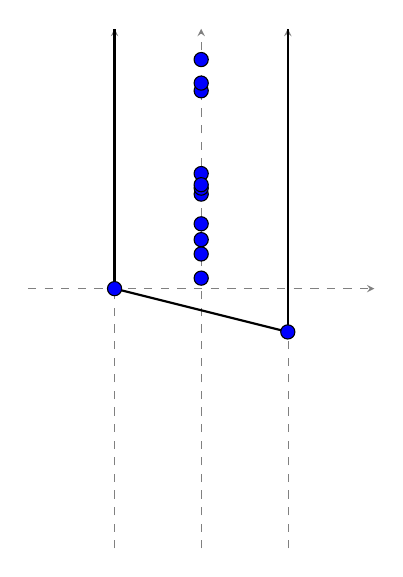
\begin{tikzpicture}[>=stealth, x=1.1cm, y=1.1cm]
            % Dashed lines (axes)
            \draw[help lines, dashed, ->] (-1,0) -- (3,0);
            \draw[help lines, dashed, ->] (0,-3) -- (0,3);
            \draw[help lines, dashed, ->] (1,-3) -- (1,3);
            \draw[help lines, dashed, ->] (2,-3) -- (2,3);
            \draw[thick] (0,0) -- (0,3);
            \draw[thick] (0,0) -- (2, -0.5);
            \draw[thick]  (2,-0.5) -- (2,3);
            \draw[thick]  (2,-0.5) -- (2,3);

            % Points (all with fill=blue and radius=0.09cm)
            \filldraw[fill=blue] (2, -0.5) circle[radius=0.09cm];
            \filldraw[fill=blue] (0, 0) circle[radius=0.09cm]; % Removed duplicate
            \filldraw[fill=blue] (1, 0.12122108098130914) circle[radius=0.09cm];
            \filldraw[fill=blue] (1, 2.28412917072110916) circle[radius=0.09cm];
            \filldraw[fill=blue] (1, 2.3729881287610001) circle[radius=0.09cm];
            \filldraw[fill=blue] (1, 0.4) circle[radius=0.09cm];
            \filldraw[fill=blue] (1, 0.5655158711807637) circle[radius=0.09cm];
            \filldraw[fill=blue] (1, 2.6445016116606668) circle[radius=0.09cm];
            \filldraw[fill=blue] (1, 0.7481703960405396) circle[radius=0.09cm];
            \filldraw[fill=blue] (1, 1.3282219276898275) circle[radius=0.09cm];
            \filldraw[fill=blue] (1, 1.0912647062501184) circle[radius=0.09cm];
            \filldraw[fill=blue] (1, 1.1603772291700336) circle[radius=0.09cm];
            \filldraw[fill=blue] (1, 1.2) circle[radius=0.09cm];
        \end{tikzpicture}~
    \end{minipage} \hspace{3cm} \begin{minipage}{.2\textwidth}
        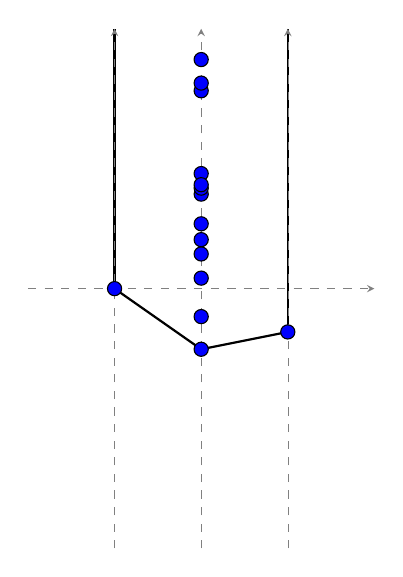
\begin{tikzpicture}[>=stealth, x=1.1cm, y=1.1cm]
            % Dashed lines (axes)
            \draw[help lines, dashed, ->] (-1,0) -- (3,0);
            \draw[thick] (0,0) -- (0,3);
            \draw[thick] (0,0) -- (1, -0.7);
            \draw[thick] (1,-0.7) -- (2,-0.5);
            \draw[thick]  (2,-0.5) -- (2,3);
            \draw[help lines, dashed, ->] (0,-3) -- (0,3);
            \draw[help lines, dashed, ->] (1,-3) -- (1,3);
            \draw[help lines, dashed, ->] (2,-3) -- (2,3);

            % Points (all with fill=blue and radius=0.09cm)
            \filldraw[fill=blue] (2, -0.5) circle[radius=0.09cm];
            \filldraw[fill=blue] (0, 0) circle[radius=0.09cm]; % Removed duplicate
            \filldraw[fill=blue] (1, -0.7) circle[radius=0.09cm];
            \filldraw[fill=blue] (1, -0.3230737092181455) circle[radius=0.09cm];
            \filldraw[fill=blue] (1, 0.12122108098130914) circle[radius=0.09cm];
            \filldraw[fill=blue] (1, 2.28412917072110916) circle[radius=0.09cm];
            \filldraw[fill=blue] (1, 2.3729881287610001) circle[radius=0.09cm];
            \filldraw[fill=blue] (1, 0.4) circle[radius=0.09cm];
            \filldraw[fill=blue] (1, 0.5655158711807637) circle[radius=0.09cm];
            \filldraw[fill=blue] (1, 2.6445016116606668) circle[radius=0.09cm];
            \filldraw[fill=blue] (1, 0.7481703960405396) circle[radius=0.09cm];
            \filldraw[fill=blue] (1, 1.3282219276898275) circle[radius=0.09cm];
            \filldraw[fill=blue] (1, 1.0912647062501184) circle[radius=0.09cm];
            \filldraw[fill=blue] (1, 1.1603772291700336) circle[radius=0.09cm];
            \filldraw[fill=blue] (1, 1.2) circle[radius=0.09cm];
        \end{tikzpicture}~
    \end{minipage}
\end{figure}
Visually, a lattice is called \textbf{semi-stable} if it satisfies the other equivalent
conditions:   If $M$ is an arbitrary sublattice of $L$ then $\mu(M) \ge \mu(L)$.


\end{document}